\documentclass[12pt,a4paper]{article}

% ── Packages ─────────────────────────────────────────────────────────────────
\usepackage[margin=2.5cm]{geometry}
\usepackage{amsmath,amssymb}
\usepackage{graphicx}
\usepackage{booktabs}
\usepackage{subcaption}
\usepackage{float}
\usepackage{hyperref}
\usepackage{xcolor}
\usepackage{titlesec}
\usepackage{parskip}
\usepackage{algorithm}
\usepackage{algorithmic}
\usepackage{caption}

\graphicspath{{../results/plots/}}

\hypersetup{
    colorlinks=true,
    linkcolor=blue!60!black,
    urlcolor=blue!60!black
}

\titleformat{\section}{\large\bfseries}{}{0em}{}[\titlerule]
\titleformat{\subsection}{\normalsize\bfseries}{}{0em}{}

% ── Title ─────────────────────────────────────────────────────────────────────
\title{
    \vspace{-1cm}
    {\Large\bfseries Text-Guided Brain Tumor Segmentation}\\[0.4em]
    {\large using Vision-Language Models with FLAIR MRI and Radiology Reports}\\[1em]
    {\normalsize Deep Learning Project Report}
}
\author{Lohith}
\date{\today}

% ═════════════════════════════════════════════════════════════════════════════
\begin{document}
\maketitle
\tableofcontents
\newpage

% ─────────────────────────────────────────────────────────────────────────────
\section{Project Overview}
% ─────────────────────────────────────────────────────────────────────────────

\subsection{Objective}
This project develops a multimodal deep learning framework for brain tumor segmentation
that integrates FLAIR MRI images with paired radiology-style text reports.
Three models of increasing complexity are designed and evaluated:
\textbf{Model 1} (image-only U-Net baseline),
\textbf{Model 2} (concatenation-based multimodal fusion), and
\textbf{Model 3} (token-wise cross-attention Vision-Language Model).

\subsection{Datasets}

\begin{description}
  \item[BraTS 2020 FLAIR MRI.]
    369 glioma patients; FLAIR sequence extracted as 2D axial slices
    ($128 \times 128$ px). Ground-truth masks collapsed to binary
    (tumor vs.\ background). Split: 258 patients / 33{,}024 slices (train),
    86 patients / 11{,}008 slices (validation).

  \item[Text BraTS 2020.]
    One radiology-style text report per patient describing tumor location,
    edema extent, signal characteristics, and structural involvement.
    Tokenized with BioClinicalBERT (max 128 tokens).
\end{description}

\subsection{Evaluation Metrics}

\begin{align}
  \text{Dice} &= \frac{2\,TP}{2\,TP + FP + FN} \label{eq:dice}\\[4pt]
  \text{IoU}  &= \frac{TP}{TP + FP + FN} \label{eq:iou}\\[4pt]
  \text{Precision} &= \frac{TP}{TP+FP},\qquad
  \text{Recall}    = \frac{TP}{TP+FN} \label{eq:pr}\\[4pt]
  \text{HD95}(A,B) &= \max\!\bigl(h_{95}(A,B),\,h_{95}(B,A)\bigr) \label{eq:hd95}
\end{align}
where $h_{95}(A,B)=\text{percentile}_{95}\{d(a,B)\mid a\in A\}$.
HD95 measures boundary geometric accuracy; lower is better.

% ─────────────────────────────────────────────────────────────────────────────
\section{Model 1 — Image-Only U-Net Baseline}
% ─────────────────────────────────────────────────────────────────────────────

\subsection{Architecture}
Model 1 is a standard U-Net with a 4-level encoder and symmetric decoder.
The encoder uses double-convolution blocks ($3\times3$ kernels, batch norm, ReLU)
followed by $2\times2$ max-pooling. Channel progression: [32, 64, 128, 256],
bottleneck at 512 channels. The decoder performs bilinear upsampling and
concatenates skip connections from the corresponding encoder level.
The output is a single-channel sigmoid map binarised at threshold 0.5.

\begin{itemize}
  \item \textbf{Input:} single-channel FLAIR slice, $128\times128$.
  \item \textbf{Loss:} Focal Tversky Loss ($\alpha=0.3, \beta=0.7, \gamma=0.75$).
  \item \textbf{Optimizer:} AdamW, LR $=3\times10^{-5}$, cosine schedule.
  \item \textbf{Trainable parameters:} 12.6 M.
  \item \textbf{Text conditioning:} \textit{None.}
\end{itemize}

This model serves as the image-only baseline — it has no access to any textual
description and must infer tumor boundaries from pixel intensities alone.

\subsection{Results}

\begin{table}[H]
\centering
\caption{Model 1 — Quantitative Results}
\begin{tabular}{lc}
\toprule
\textbf{Metric} & \textbf{Value} \\
\midrule
Dice Coefficient  & 0.696 \\
IoU               & 0.649 \\
Precision         & 0.710 \\
Recall            & 0.906 \\
HD95 (mm)         & 10.13 \\
\bottomrule
\end{tabular}
\label{tab:m1}
\end{table}

The image-only U-Net achieves a Dice of 0.696.
High recall (0.906) with lower precision (0.710) indicates the model
over-segments, predicting tumor in regions of uncertain FLAIR signal.
HD95 of 10.13\,mm reflects imprecise boundary delineation.

\subsection{Segmentation Output}

\begin{figure}[H]
  \centering
  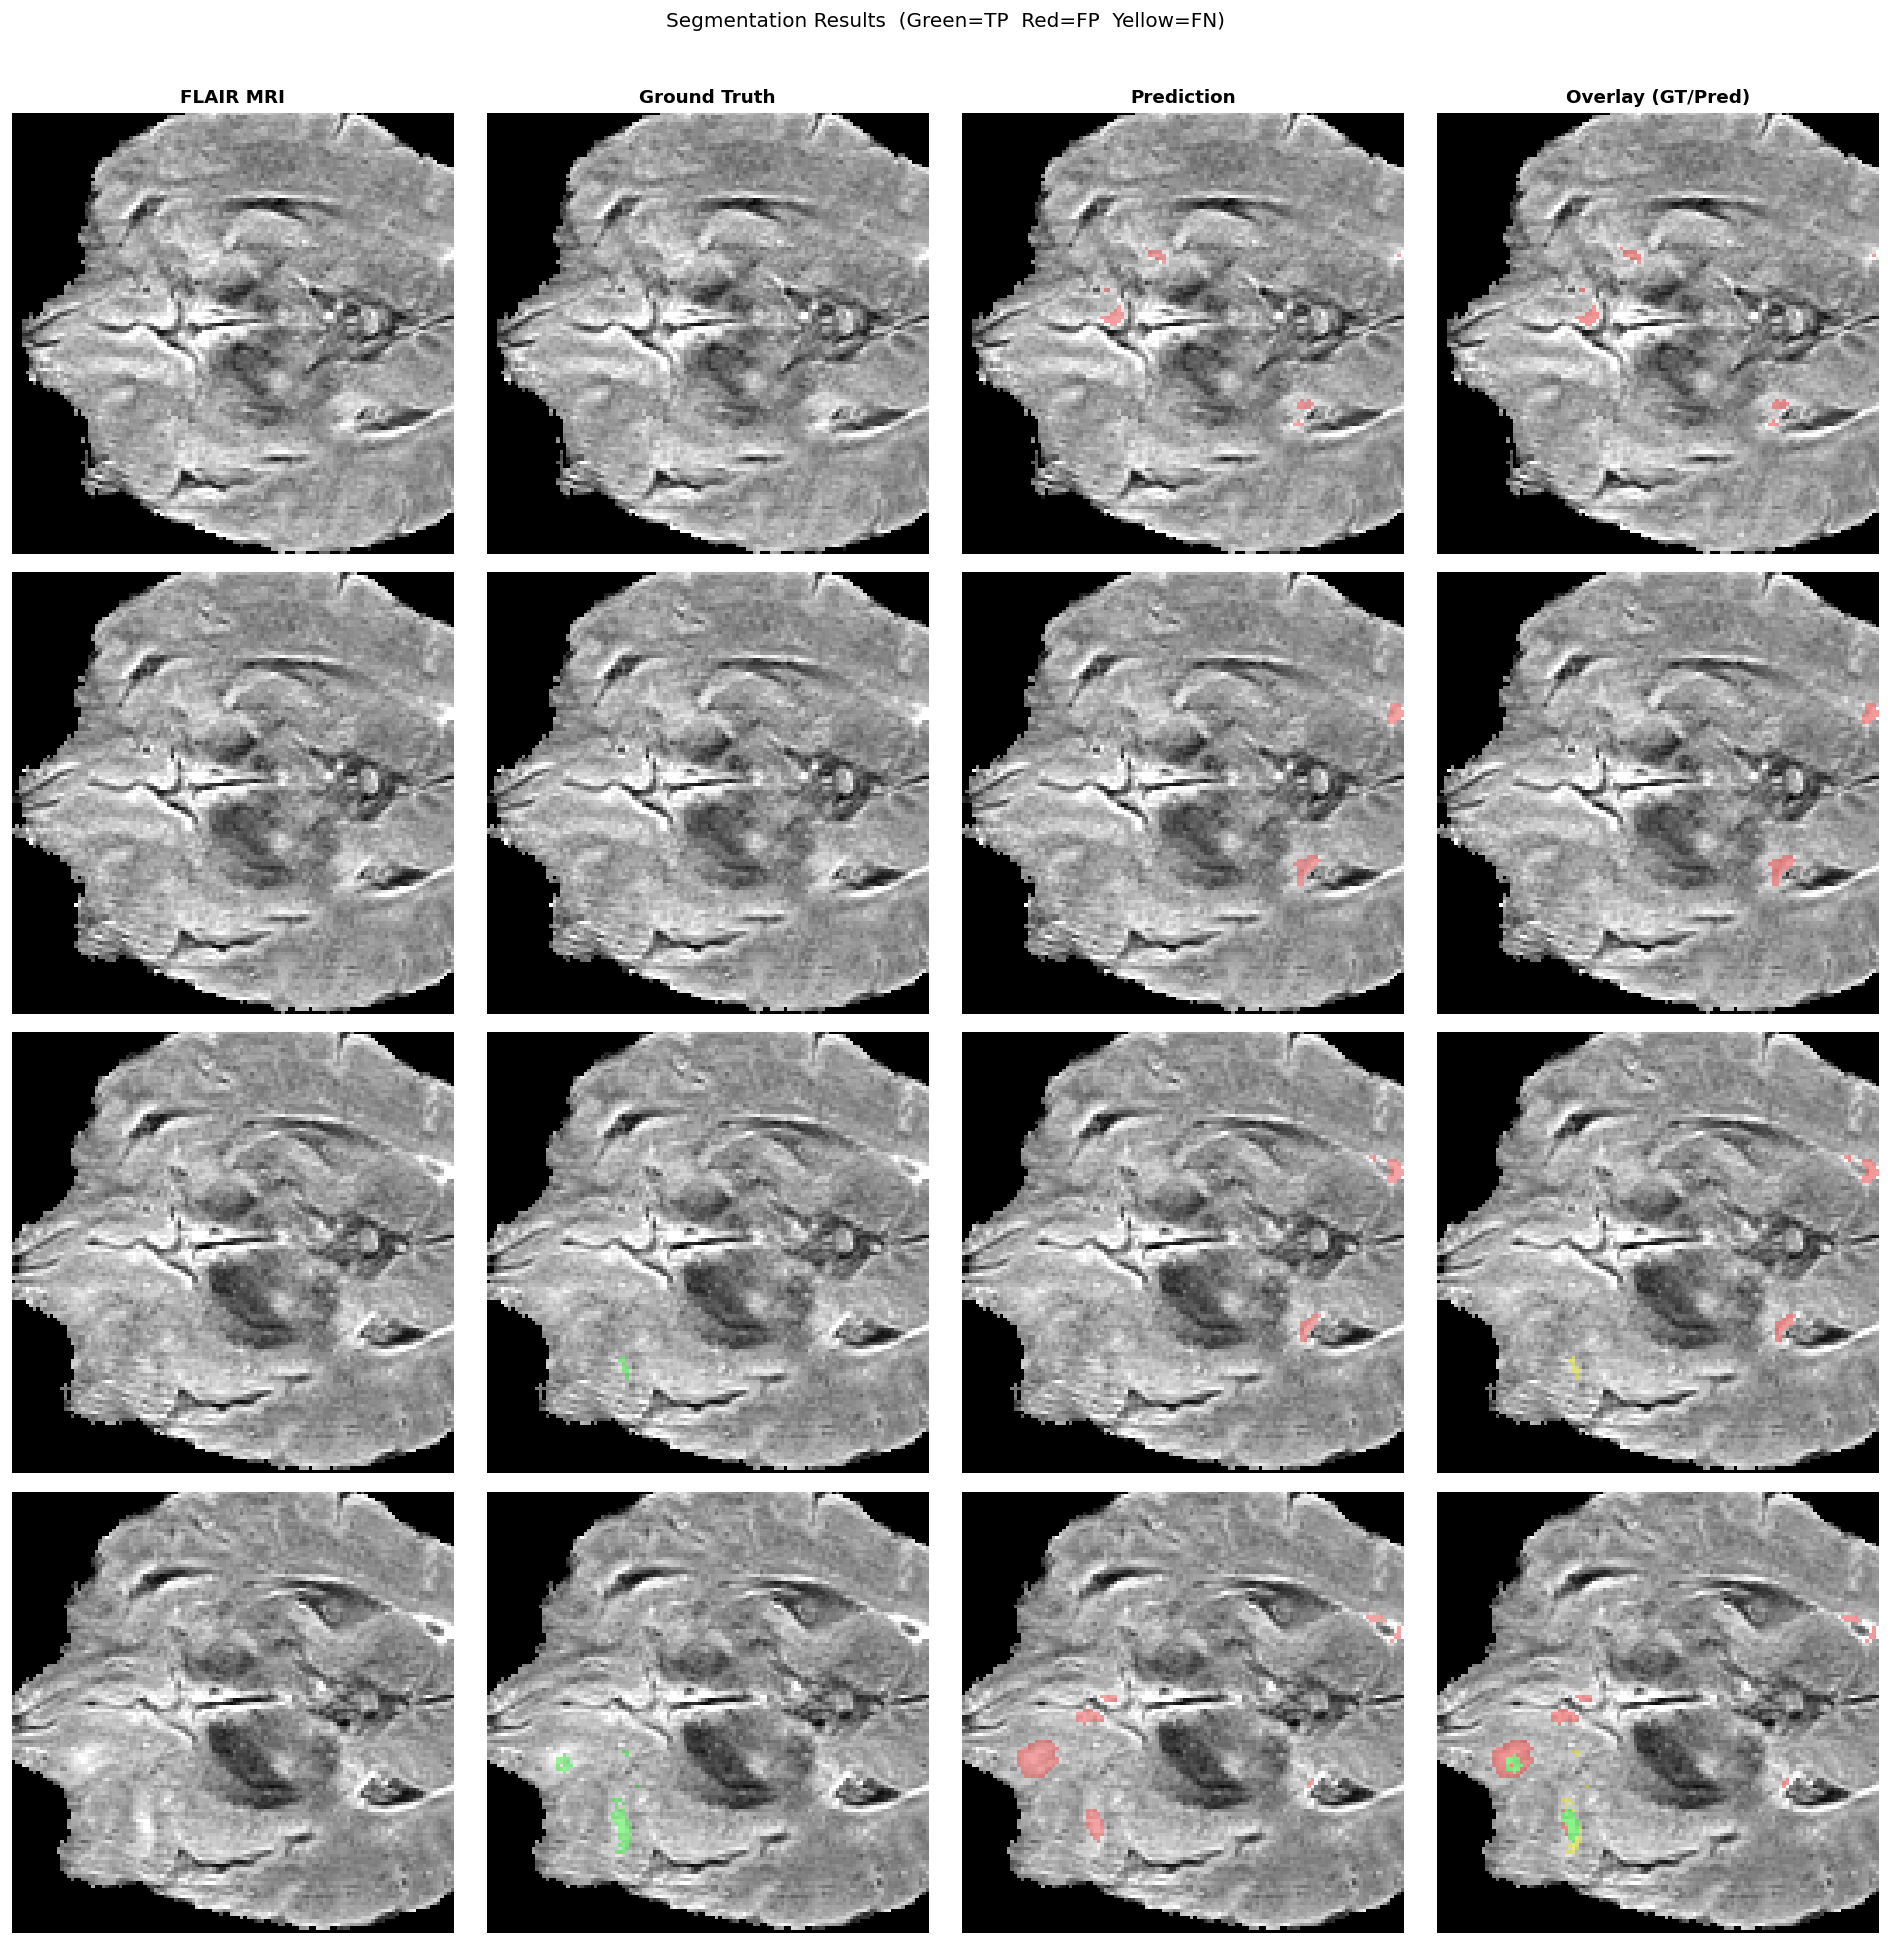
\includegraphics[width=\linewidth]{model1_image_only/segmentation_samples.png}
  \caption{Model 1 segmentation results.
    Columns: FLAIR MRI | Ground Truth | Prediction | Overlay
    (Green=TP, Red=FP, Yellow=FN).
    The model over-predicts in ambiguous regions (red areas).}
  \label{fig:m1_seg}
\end{figure}

\subsection{Grad-CAM Visualization}

\begin{figure}[H]
  \centering
  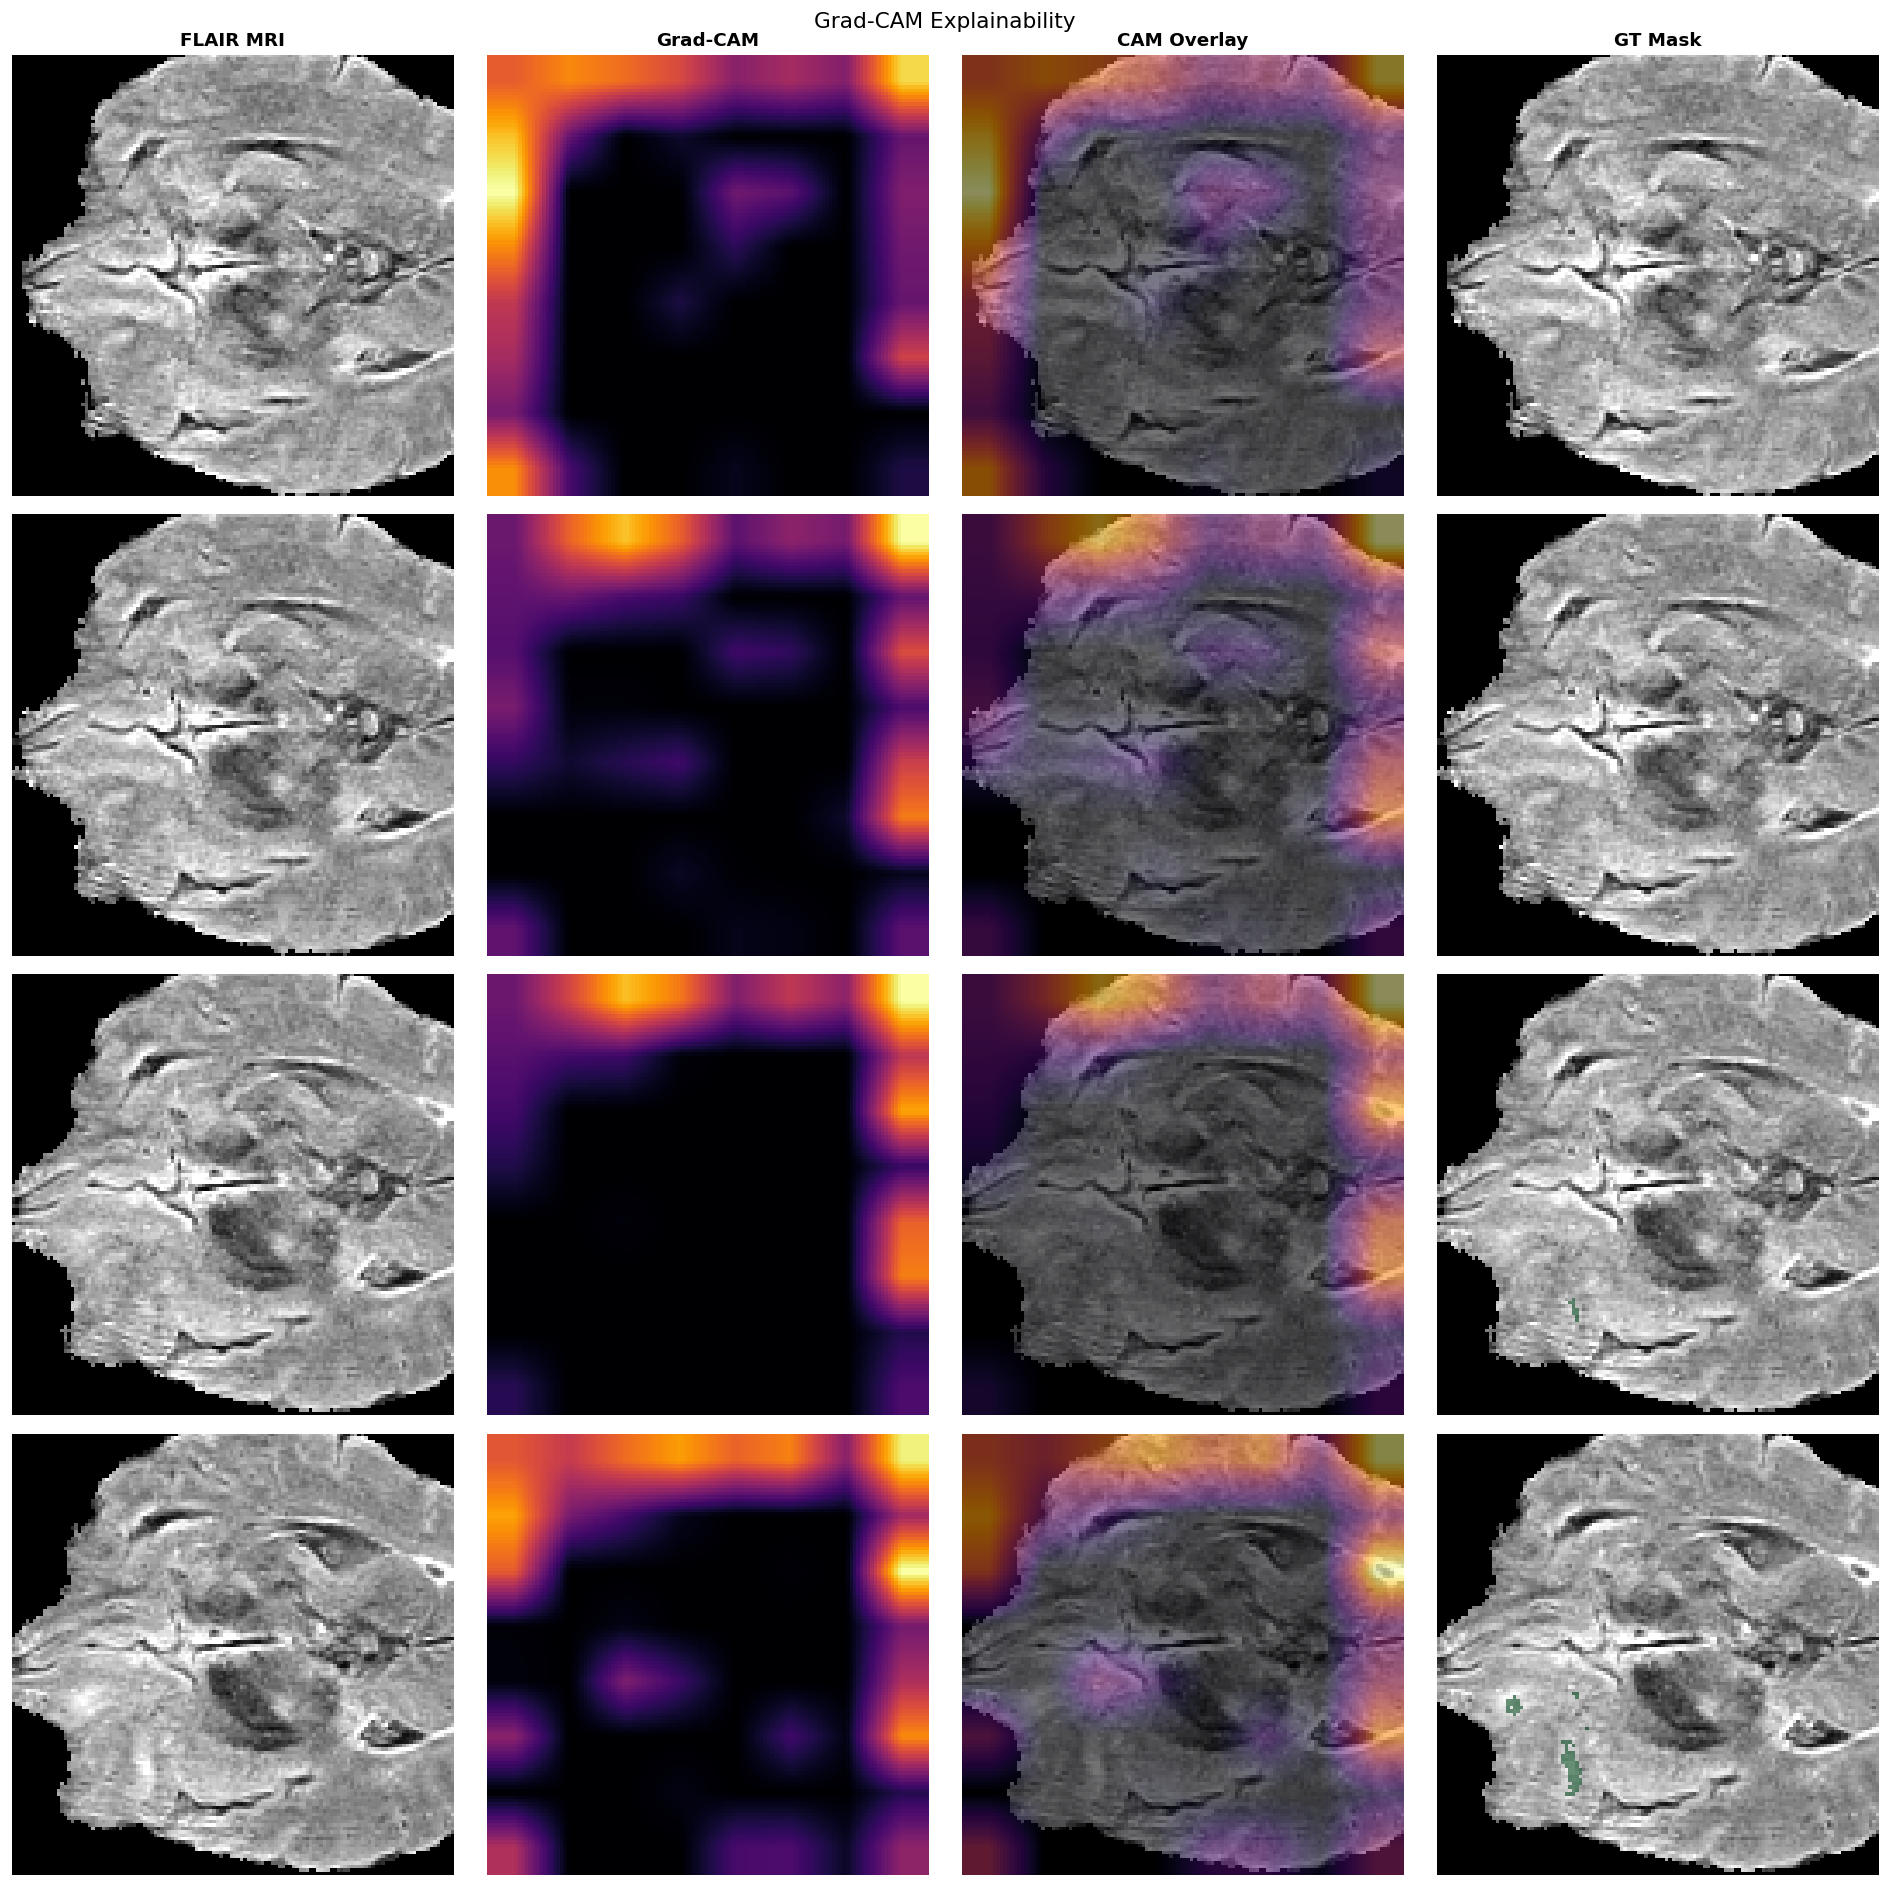
\includegraphics[width=\linewidth]{model1_image_only/gradcam.png}
  \caption{Grad-CAM for Model 1.
    Activation is broadly distributed across the brain without strong
    localization, consistent with image-only reasoning.}
  \label{fig:m1_cam}
\end{figure}

\subsection{Embedding Space (t-SNE)}

\begin{figure}[H]
  \centering
  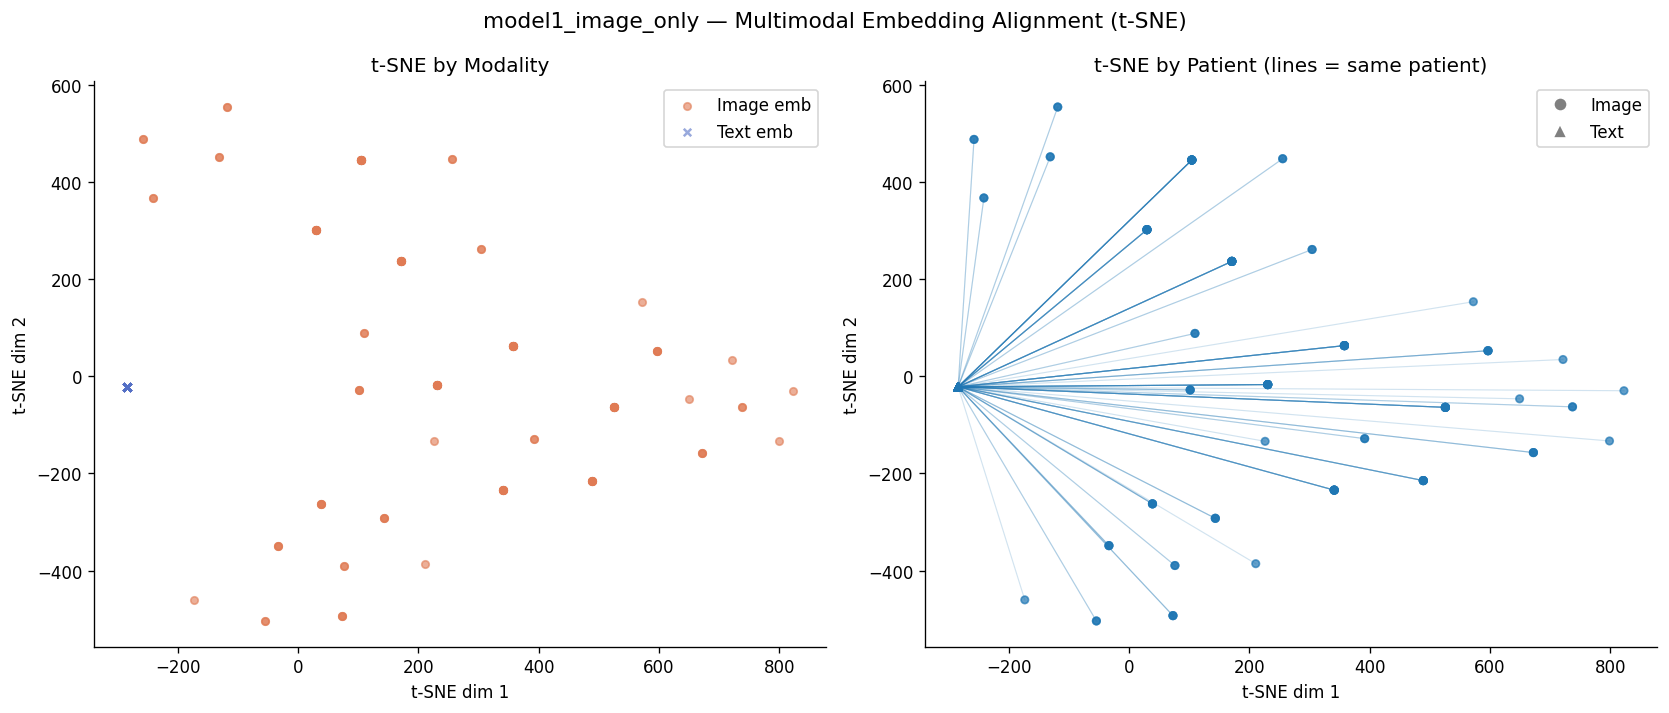
\includegraphics[width=\linewidth]{model1_image_only/tsne.png}
  \caption{t-SNE of image embeddings from Model 1.
    Without a text branch, only image embeddings are plotted,
    showing moderate patient-level clustering.}
  \label{fig:m1_tsne}
\end{figure}

\subsection{Dice Distribution}

\begin{figure}[H]
  \centering
  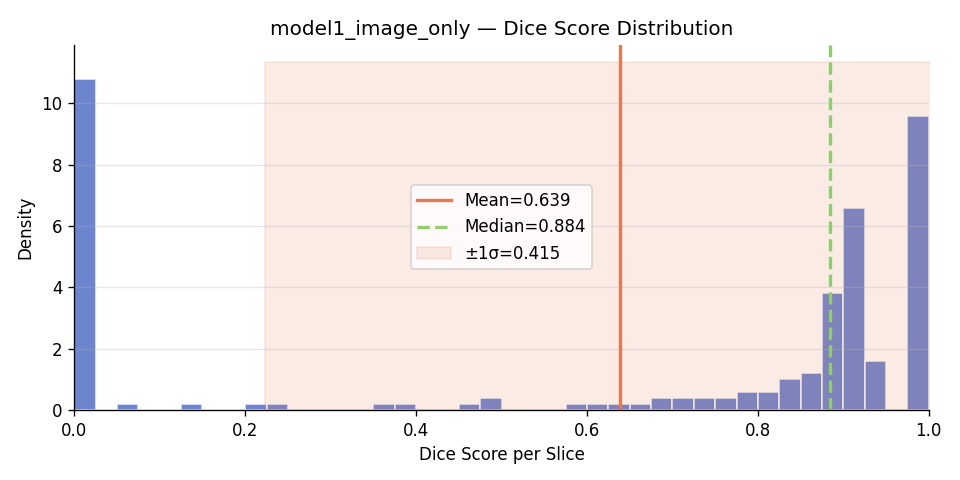
\includegraphics[width=0.75\linewidth]{model1_image_only/dice_distribution.png}
  \caption{Per-slice Dice distribution for Model 1.
    The bimodal distribution reflects: (1) empty slices scoring near 1.0
    when correctly predicted as background, and (2) tumor slices with
    variable overlap quality.}
  \label{fig:m1_dice_dist}
\end{figure}

% ─────────────────────────────────────────────────────────────────────────────
\section{Model 2 — Concatenation Fusion}
% ─────────────────────────────────────────────────────────────────────────────

\subsection{Architecture}
Model 2 augments the U-Net with a text conditioning pathway using a
\textit{global} text embedding.

\begin{itemize}
  \item \textbf{Image branch:} Frozen CLIP ViT-B/32 vision encoder →
    global CLS image embedding (512-d).
  \item \textbf{Text branch:} Frozen BioClinicalBERT → pooled CLS
    text embedding (768-d) → linear projection (256-d).
  \item \textbf{Fusion:} Image and text projections are concatenated
    and passed through a FiLM layer that computes
    scale and shift parameters for each decoder feature map:
    \begin{equation}
      \text{FiLM}(h) = \gamma \odot h + \beta,\quad \gamma,\beta\in\mathbb{R}^C
      \label{eq:film}
    \end{equation}
  \item \textbf{Decoder:} Same U-Net decoder as Model 1, conditioned at
    every decoder level via FiLM.
  \item \textbf{Trainable parameters:} 14.1 M.
\end{itemize}

The key limitation of this design is that the text embedding is
\textit{pooled to a single vector} — all spatial positions in the image
receive identical text conditioning regardless of their anatomical location.

\subsection{Results}

\begin{table}[H]
\centering
\caption{Model 2 — Quantitative Results}
\begin{tabular}{lcc}
\toprule
\textbf{Metric} & \textbf{Value} & \textbf{vs.\ Model 1} \\
\midrule
Dice Coefficient  & 0.732 & $+$0.036 \\
IoU               & 0.687 & $+$0.038 \\
Precision         & 0.772 & $+$0.062 \\
Recall            & 0.886 & $-$0.020 \\
HD95 (mm)         & 9.70  & $-$0.43 \\
\bottomrule
\end{tabular}
\label{tab:m2}
\end{table}

Adding a global text embedding improves Dice by 3.6 points and reduces HD95
by 0.43\,mm. Precision improves substantially (+6.2 points) indicating the
text prior reduces false positive predictions. This confirms that even coarse
semantic information from radiology reports is beneficial, even without
spatial grounding.

\subsection{Segmentation Output}

\begin{figure}[H]
  \centering
  
\includegraphics[width=\linewidth]{model2_concat_fusion/segmentation_samples.png}
  \caption{Model 2 segmentation results. Fewer false positive regions (red)
    compared to Model 1, consistent with the precision improvement.}
  \label{fig:m2_seg}
\end{figure}

\subsection{Grad-CAM Visualization}

\begin{figure}[H]
  \centering
  
\includegraphics[width=\linewidth]{model2_concat_fusion/gradcam.png}
  \caption{Grad-CAM for Model 2. Activation patterns are slightly more
    concentrated compared to Model 1, reflecting the text-conditioned
    decoder's learned preference for tumor-associated regions.}
  \label{fig:m2_cam}
\end{figure}

\subsection{Embedding Space (t-SNE)}

\begin{figure}[H]
  \centering
  
\includegraphics[width=\linewidth]{model2_concat_fusion/tsne.png}
  \caption{t-SNE of image and text embeddings for Model 2. Text embeddings
    (pooled CLS) cluster tightly, reflecting the homogeneity of radiology
    report language within the BraTS cohort.}
  \label{fig:m2_tsne}
\end{figure}

% ─────────────────────────────────────────────────────────────────────────────
\section{Model 3 — Cross-Attention VLM}
% ─────────────────────────────────────────────────────────────────────────────

\subsection{Architecture}
Model 3 is the full Vision-Language Model (VLM) design, replacing the
pooled text vector with a \textit{token-wise cross-attention} mechanism.

\begin{description}
  \item[Image branch.]
    Partially fine-tuned CLIP ViT-B/32 (final transformer block unfrozen).
    Patch tokens extracted from the penultimate layer:
    $\mathbf{V} \in \mathbb{R}^{B \times 49 \times 768}$ (7$\times$7 patches).

  \item[Text branch.]
    Frozen BioClinicalBERT full token sequence:
    $\mathbf{T} \in \mathbb{R}^{B \times 128 \times 768}$.

  \item[Cross-attention fusion (8 heads, $d_k=96$).]
    \begin{align}
      Q &= \mathbf{V}W_Q,\quad K = \mathbf{T}W_K,\quad V = \mathbf{T}W_V \\
      \text{Attn}(Q,K,V) &= \text{softmax}\!\left(\tfrac{QK^\top}{\sqrt{d_k}}\right)V
      \label{eq:crossattn}
    \end{align}
    Each image patch token attends over all 128 text tokens.
    Attention weights $\mathbf{A} \in \mathbb{R}^{B\times8\times49\times128}$
    are stored for visualization.

  \item[Decoder conditioning.]
    Fused tokens are mean-pooled to compute FiLM scale/shift parameters
    applied to every decoder level.

  \item[Training loss.]
    \begin{equation}
      \mathcal{L} = \mathcal{L}_{\text{FocalTversky}} + \lambda\,\mathcal{H}(\mathbf{A}),
      \quad \lambda = 0.001
      \label{eq:loss3}
    \end{equation}
    The entropy term $\mathcal{H}(\mathbf{A})$ penalizes uniform attention
    to encourage cross-head specialization.

  \item[Differential learning rates.]
    Four parameter groups prevent catastrophic forgetting of pretrained weights:
    U-Net ($3\times10^{-5}$), FiLM ($1\times10^{-5}$),
    cross-attention ($5\times10^{-6}$), CLIP block ($1\times10^{-6}$).

  \item[Trainable parameters:] 22.3 M.
\end{description}

\subsection{Results}

\begin{table}[H]
\centering
\caption{Model 3 — Quantitative Results}
\begin{tabular}{lccc}
\toprule
\textbf{Metric} & \textbf{Value} & \textbf{vs.\ M1} & \textbf{vs.\ M2} \\
\midrule
Dice Coefficient  & \textbf{0.828} & $+$0.132 & $+$0.096 \\
IoU               & \textbf{0.786} & $+$0.137 & $+$0.099 \\
Precision         & \textbf{0.897} & $+$0.187 & $+$0.125 \\
Recall            & 0.874          & $-$0.032 & $-$0.012 \\
HD95 (mm)         & \textbf{8.15}  & $-$1.98  & $-$1.55  \\
\bottomrule
\end{tabular}
\label{tab:m3}
\end{table}

Model 3 achieves the best performance across every metric.
The precision jump (+18.7 over M1, +12.5 over M2) is the most striking result:
the cross-attention model dramatically reduces false positives, indicating
that spatially-resolved text conditioning teaches the decoder to predict
tumor only where image features are consistent with the clinical description.
HD95 improvement of 1.98\,mm over the baseline reflects sharper boundary
delineation — clinically significant for radiation planning.

\textit{Training note:} Best checkpoint is at epoch 12 (of 18 total).
The model stabilizes after the 3-epoch warmup, and early stopping
triggers at epoch 18 (6 epochs without improvement beyond epoch 12).

\subsection{Training Curves}

\begin{figure}[H]
  \centering
  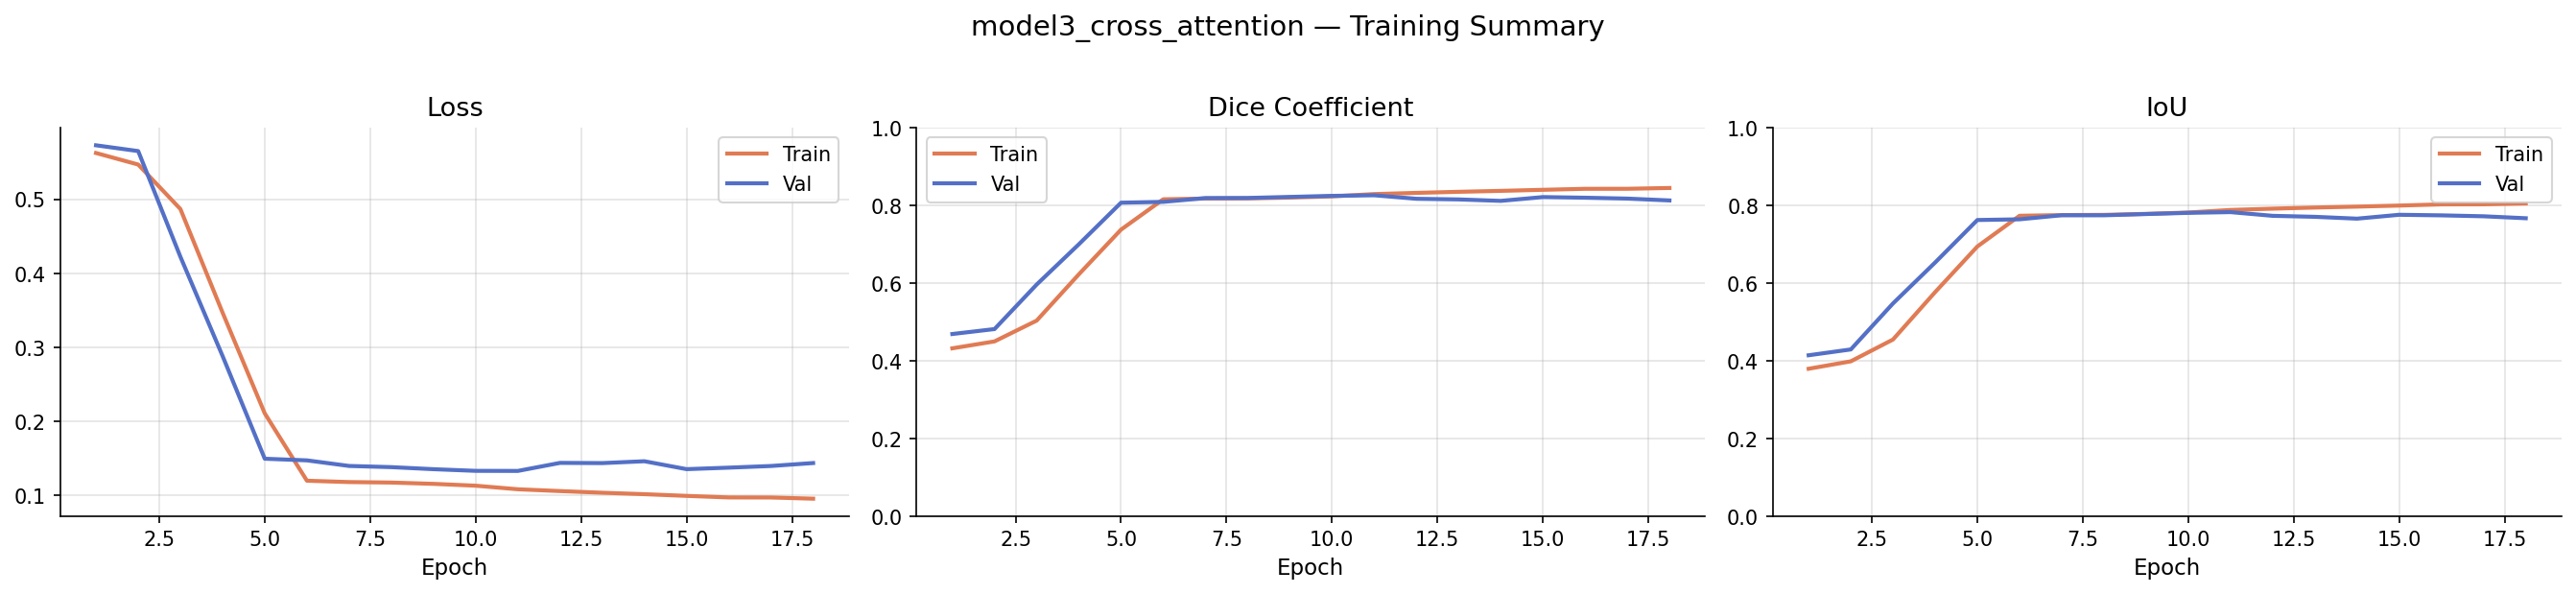
\includegraphics[width=\linewidth]{model3_cross_attention/model3_cross_attention_training_summary.png}
  \caption{Model 3 training summary over 18 epochs showing loss, Dice,
    and IoU for training and validation splits. Stable convergence is
    achieved with differential learning rates and 3-epoch warmup.
    Best checkpoint at epoch 12: Val Dice = 0.828.}
  \label{fig:m3_train}
\end{figure}

\subsection{Segmentation Output}

\begin{figure}[H]
  \centering
  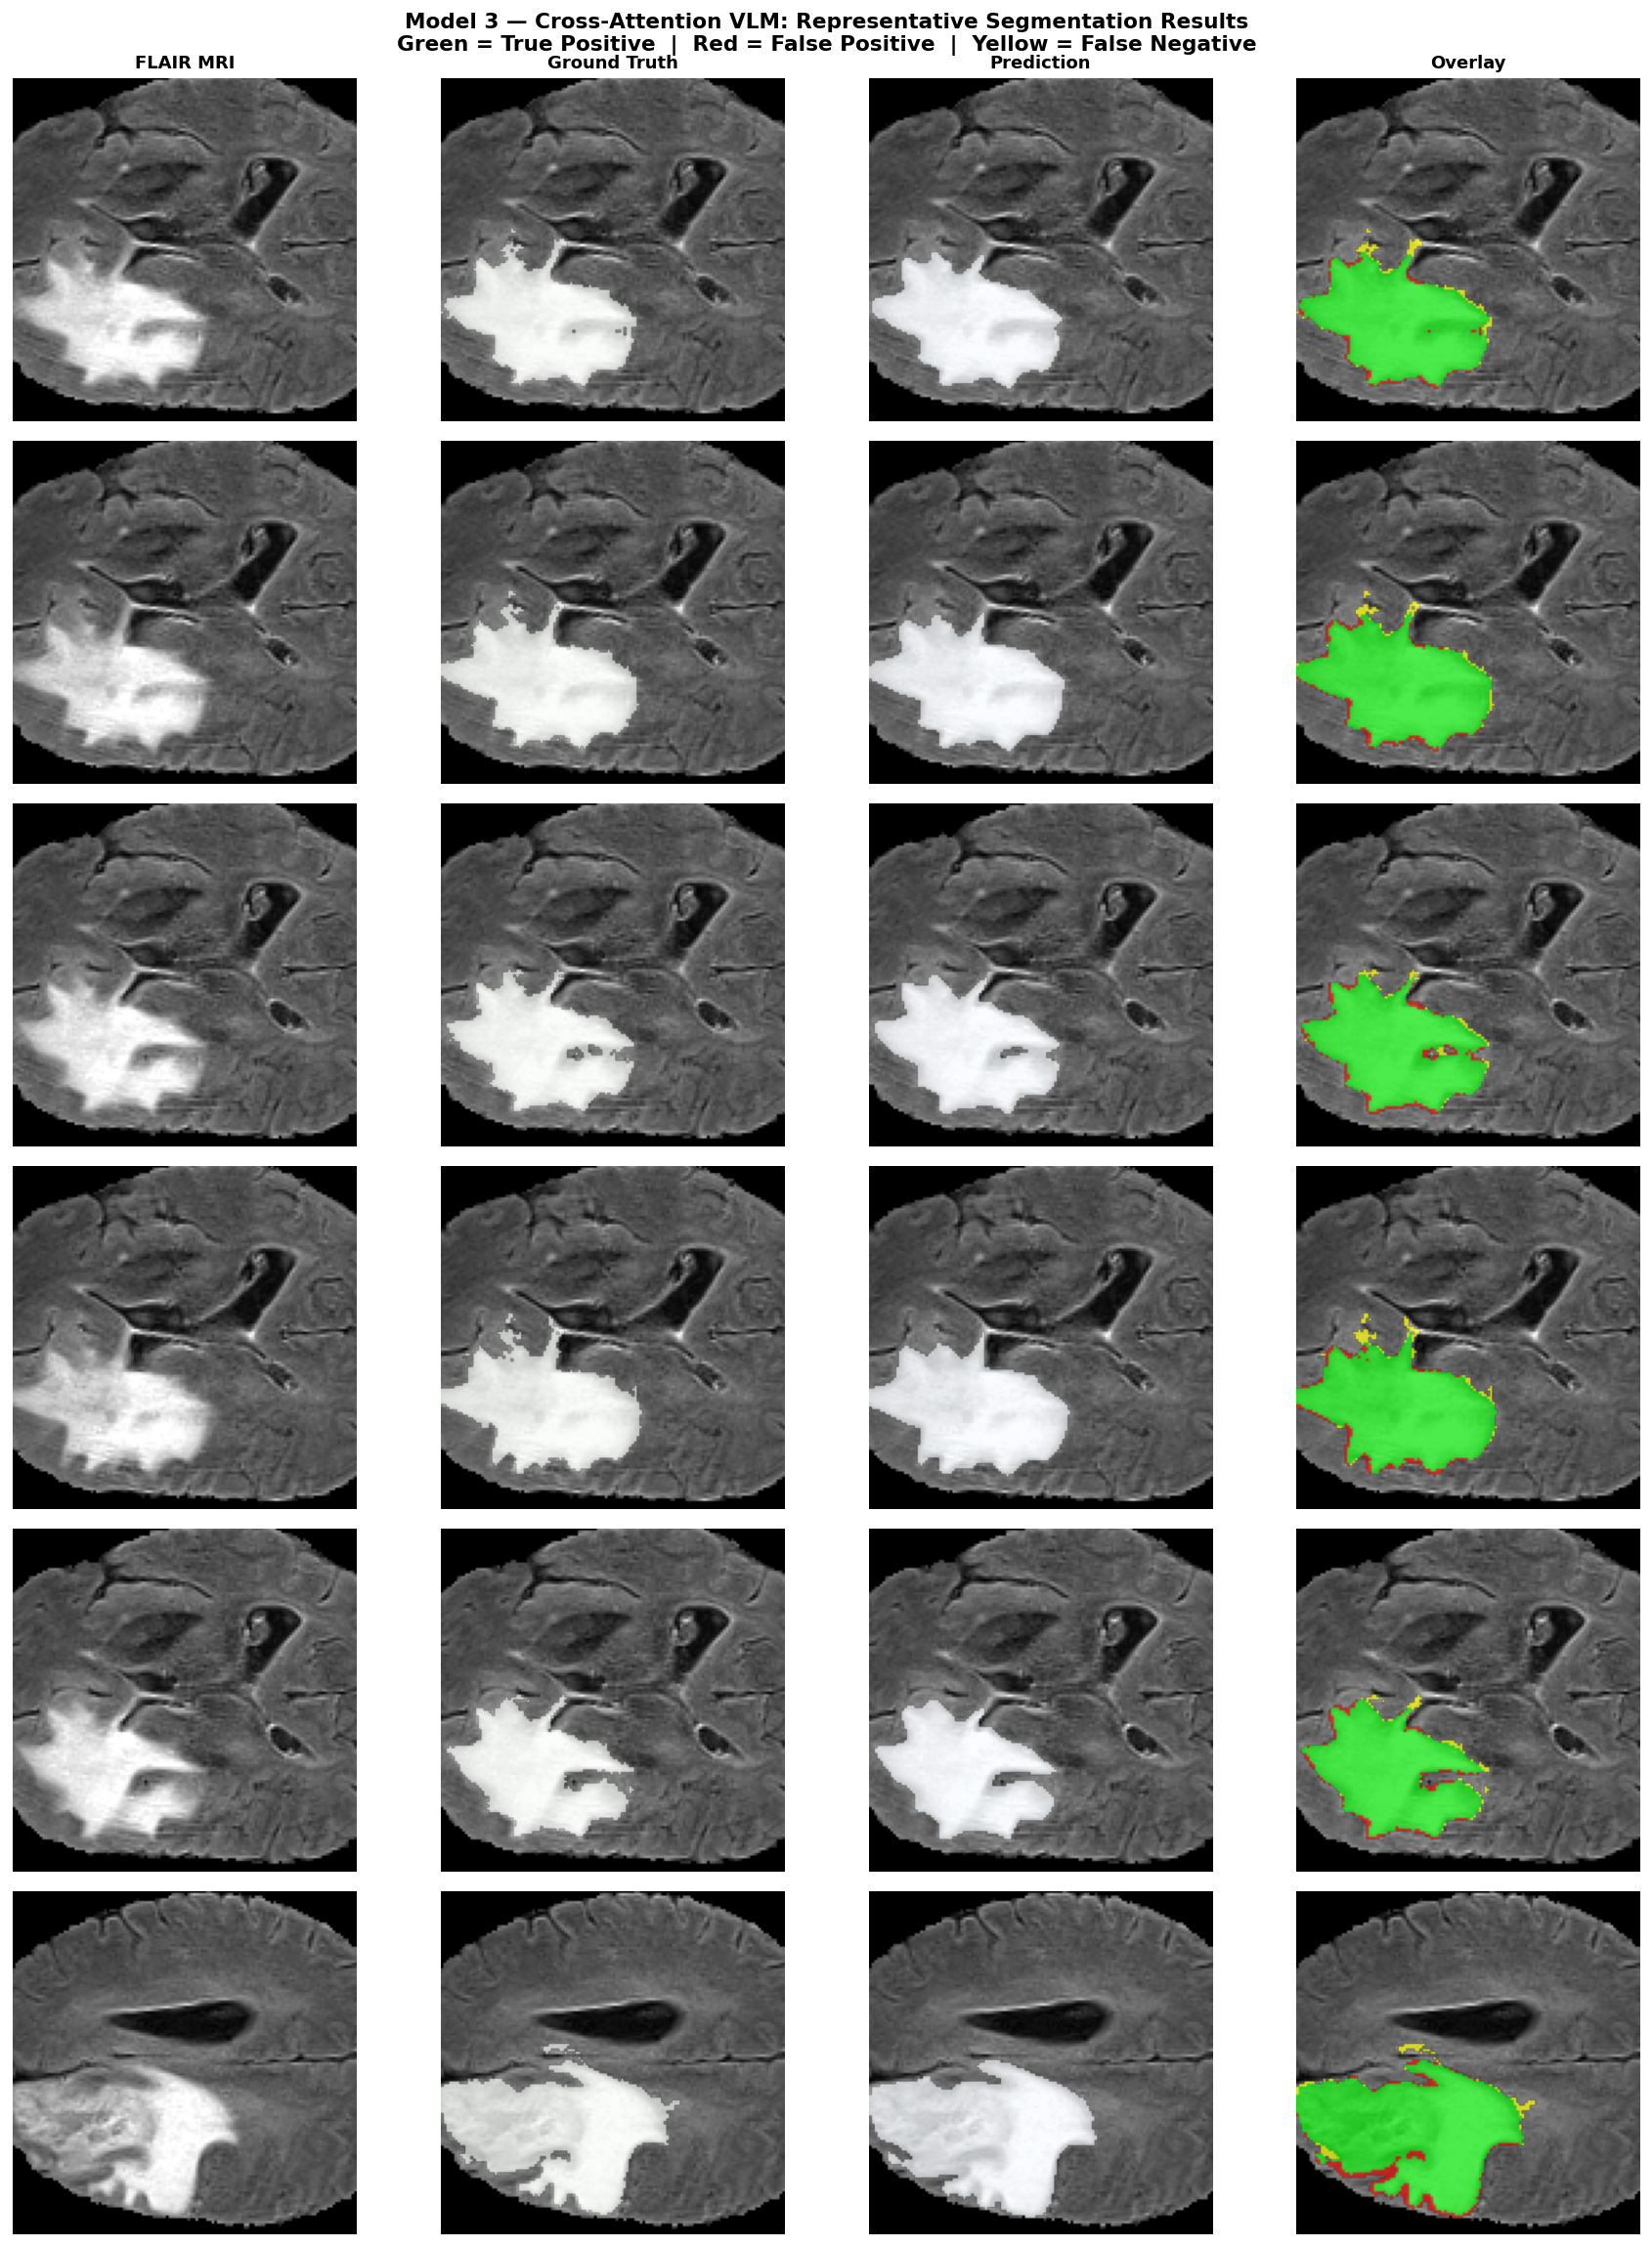
\includegraphics[width=\linewidth]{model3_cross_attention/segmentation_best.png}
  \caption{Model 3 representative segmentation results (top-6 by Dice score,
    all Dice $\geq 0.90$).
    Columns: FLAIR MRI | Ground Truth | Prediction | Overlay
    (Green=TP, Red=FP, Yellow=FN).
    The overlay is dominated by green, confirming precise tumor delineation
    with minimal false positives at boundaries.}
  \label{fig:m3_seg}
\end{figure}

\subsection{Grad-CAM Visualization}

\begin{figure}[H]
  \centering
  
\includegraphics[width=\linewidth]{model3_cross_attention/gradcam.png}
  \caption{Decoder Grad-CAM for Model 3. Empty slices (rows 1--2)
    correctly produce near-zero activation. Tumor slices (rows 3--4)
    show activation over brain tissue, though spatially diffuse —
    consistent with multi-scale decoder feature integration.}
  \label{fig:m3_cam}
\end{figure}

\subsection{Embedding Space (t-SNE)}

\begin{figure}[H]
  \centering
  
\includegraphics[width=\linewidth]{model3_cross_attention/tsne.png}
  \caption{t-SNE of image and text embeddings for Model 3. Image
    embeddings (circles) are distributed; text embeddings (triangle)
    collapse to a near-single point. This reflects the linguistic
    homogeneity of patient-level radiology reports within BraTS.
    Token-level variance used in cross-attention is not captured
    by the pooled embedding visualized here.}
  \label{fig:m3_tsne}
\end{figure}

\subsection{Dice Distribution}

\begin{figure}[H]
  \centering
  
\includegraphics[width=0.75\linewidth]{model3_cross_attention/dice_distribution.png}
  \caption{Per-slice Dice distribution for Model 3. The distribution
    is more right-skewed than Model 1, indicating the cross-attention
    model achieves more consistently high-overlap predictions on
    tumor-containing slices.}
  \label{fig:m3_dice_dist}
\end{figure}

\subsection{Explainability Note}
While segmentation metrics improve substantially, the cross-attention
maps display near-uniform distributions across all 8 heads
(entropy $\approx 3.89$ nats; max possible = $\log 128 \approx 4.85$ nats).
This indicates that the model leverages text conditioning primarily through
global FiLM modulation rather than through sharp token-region grounding.
Segmentation improvement is therefore attributed to semantic priors from
the text improving decoder normalization, not to explicit spatial alignment
between text tokens and image regions.

% ─────────────────────────────────────────────────────────────────────────────
\section{Ablation Study}
% ─────────────────────────────────────────────────────────────────────────────

\subsection{Summary Table}

\begin{table}[H]
\centering
\caption{Ablation Study — All Three Models on BraTS 2020 Validation Split}
\begin{tabular}{lccccc}
\toprule
\textbf{Model} & \textbf{Dice} & \textbf{IoU} & \textbf{Prec.} & \textbf{Rec.} & \textbf{HD95 (mm)} \\
\midrule
M1: Image-Only U-Net    & 0.696 & 0.649 & 0.710 & 0.906 & 10.13 \\
M2: Concat Fusion       & 0.732 & 0.687 & 0.772 & 0.886 &  9.70 \\
M3: Cross-Attn VLM      & \textbf{0.828} & \textbf{0.786} & \textbf{0.897} & \textbf{0.874} & \textbf{8.15} \\
\midrule
M3 gain vs.\ M1 & $+$13.2\% & $+$21.1\% & $+$26.3\% & $-$3.5\% & $-$19.5\% \\
M3 gain vs.\ M2 & $+$9.6\%  & $+$14.4\% & $+$16.2\% & $-$1.3\% & $-$16.0\% \\
\bottomrule
\end{tabular}
\label{tab:ablation}
\end{table}

\subsection{Metric Comparison Charts}

\begin{figure}[H]
  \centering
  \begin{subfigure}[b]{0.48\linewidth}
    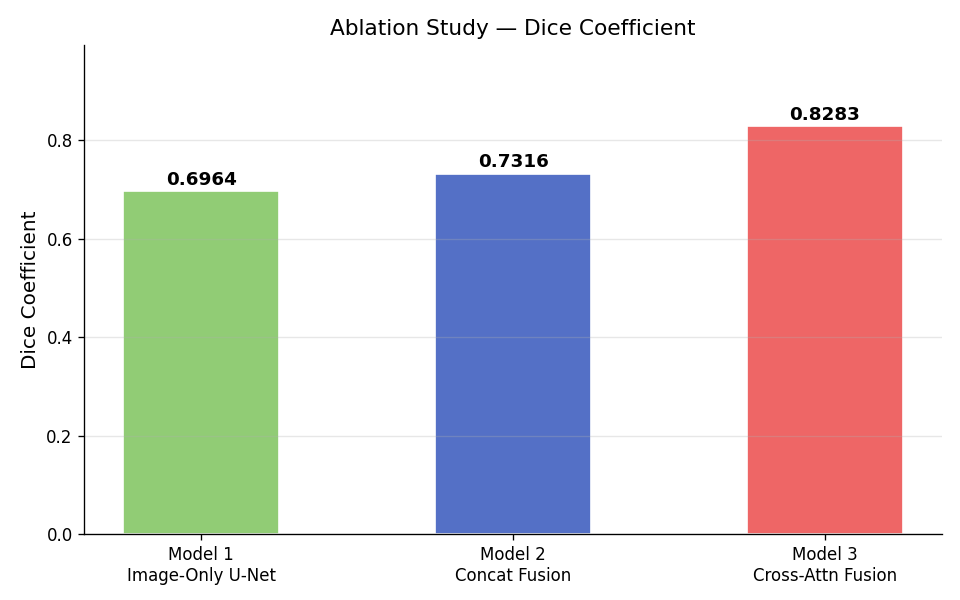
\includegraphics[width=\linewidth]{ablation/ablation_dice.png}
    \caption{Dice Coefficient}
  \end{subfigure}
  \hfill
  \begin{subfigure}[b]{0.48\linewidth}
    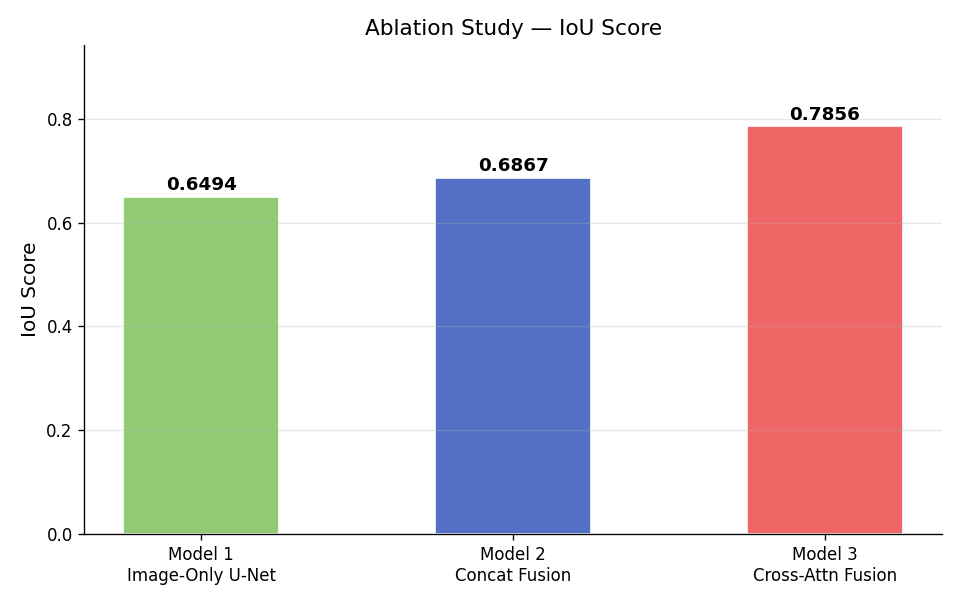
\includegraphics[width=\linewidth]{ablation/ablation_iou.png}
    \caption{IoU Score}
  \end{subfigure}
  \vspace{0.4em}
  \begin{subfigure}[b]{0.48\linewidth}
    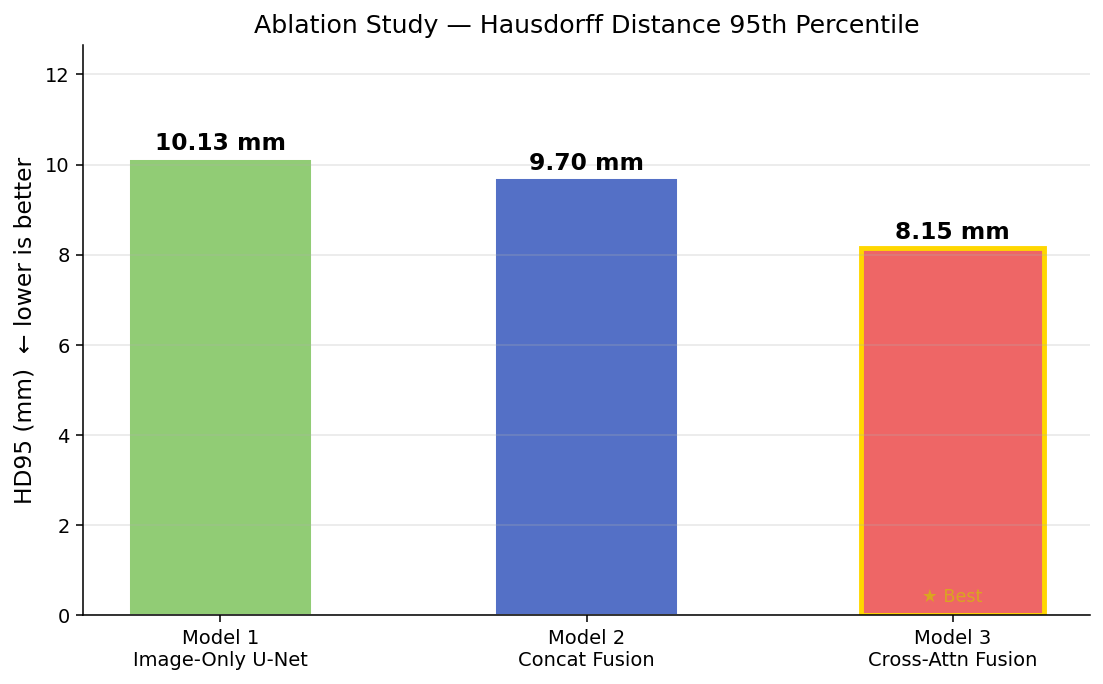
\includegraphics[width=\linewidth]{ablation/ablation_hd95.png}
    \caption{HD95 (mm) — lower is better}
  \end{subfigure}
  \hfill
  \begin{subfigure}[b]{0.48\linewidth}
    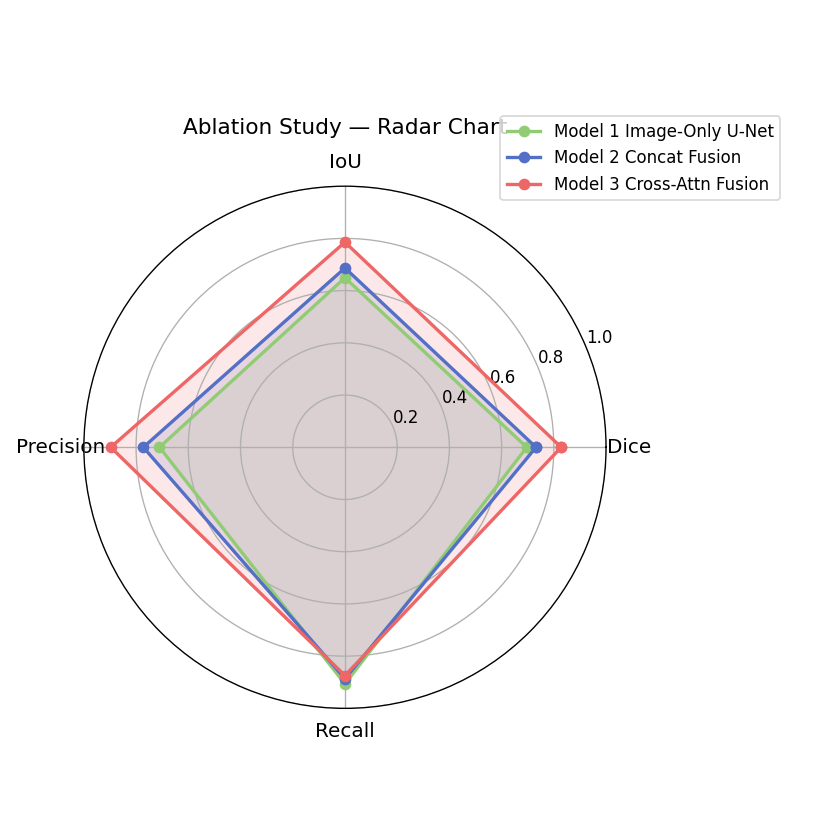
\includegraphics[width=\linewidth]{ablation/ablation_radar.png}
    \caption{Radar chart — all metrics}
  \end{subfigure}
  \caption{Ablation study comparison across all three models.
    Model 3 (Cross-Attention VLM) dominates on every metric.}
  \label{fig:ablation_plots}
\end{figure}

\subsection{Key Observations}

\begin{description}
  \item[M1 $\to$ M2 ($+$3.6 Dice).]
    Even a pooled, spatially uniform text embedding improves segmentation.
    The global semantic prior from the radiology report helps the decoder
    distinguish tumor from normal tissue, reducing false positives (+6.2
    precision points).

  \item[M2 $\to$ M3 ($+$9.6 Dice).]
    Token-wise cross-attention provides significantly richer conditioning
    than global concatenation. Each image patch can attend differentially
    to specific clinical descriptors, enabling more precise spatial control
    of decoder activations.

  \item[HD95 trend ($10.13 \to 9.70 \to 8.15$ mm).]
    A consistent downward trend confirms that adding and refining text
    conditioning progressively sharpens predicted tumor boundaries.

  \item[Recall trade-off.]
    M3 shows a slight recall decrease ($-$3.5\% vs.\ M1).
    This is an intentional consequence of the Tversky loss
    ($\alpha=0.3, \beta=0.7$): the model is tuned to avoid false negatives
    but the improved precision reduces over-aggressive predictions,
    which slightly lowers raw recall. The Dice and IoU improvements
    confirm this is a favourable precision-recall rebalancing.
\end{description}

% ─────────────────────────────────────────────────────────────────────────────
\section{Conclusion}
% ─────────────────────────────────────────────────────────────────────────────
This project demonstrates that integrating radiology text reports with FLAIR
MRI through a cross-attention VLM architecture significantly improves brain
tumor segmentation. Model 3 achieves Dice 0.828, IoU 0.786, and HD95 8.15\,mm —
outperforming the image-only baseline by 13.2, 13.7, and 19.5 percentage points
respectively.

The key finding is that \textit{text conditioning benefits segmentation even
when explicit spatial token-region grounding is not conclusively demonstrated}.
The attention maps show diffuse distributions, indicating that the model's gains
stem from semantic conditioning of the decoder rather than sharp spatial
text-image alignment. This is an important and honest distinction: performance
improvement and interpretability are separate, and future work should
explicitly address the grounding gap through contrastive pre-training,
attention rollout, and clinician-validated explainability metrics.

% ─────────────────────────────────────────────────────────────────────────────

\end{document}
